\documentclass[11pt]{article}
\usepackage[margin=1in]{geometry}
\usepackage{booktabs}
\usepackage{amsmath}
\usepackage{graphicx}

\title{Characteristic-Time Grid Study\\ Mass at $t^{*}$ versus Grid Size}
\date{18 August 2026, extended to $224 \times 224$ on 26 August 2026}
\author{}

\begin{document}
\maketitle

\section*{Parameters}

\noindent
Held fixed across every grid:

\medskip
\noindent
\begin{tabular}{ll}
\toprule
Microtubules & $N = 16$ \\
Advective velocity & $v = 10^{4}$ \\
Switch rates & $a = b = w = 100$ \\
Dimensionless solution time & $T = 1$ \\
Domain radius & $R = 1.0$ \\
Diffusion coefficient & $D = 1.0$ \\
Microtubule extraction width & $d_{\mathrm{tube}} = 0.0$ \\
Initial condition & centred \\
\bottomrule
\end{tabular}

\bigskip
\noindent
Microtubules are evenly spaced on each grid, so the ray indices are
regenerated per grid size while the count stays fixed.

\section*{Results and wall time}

\noindent
\begin{tabular}{lrrlr}
\toprule
Grid & {$t^{*}$} & {$m^{*}$} & {Device} & {Wall time} \\
\midrule
$48 \times 48$ & 0.052357 & 0.670035 & CPU & 3.8 min \\
$64 \times 64$ & 0.055390 & 0.546092 & CPU & 19.3 min \\
$80 \times 80$ & 0.057689 & 0.450505 & CPU & 1.23 hr \\
$96 \times 96$ & 0.059530 & 0.377297 & CPU & 3.68 hr \\
$112 \times 112$ & 0.061058 & 0.320804 & CPU & 9.32 hr \\
$128 \times 128$ & 0.062355 & 0.276652 & CPU & 21.31 hr \\
$144 \times 144$ & 0.063476 & 0.241655 & CPU & 43.68 hr \\
$160 \times 160$ & 0.064458 & 0.213518 & CPU & 82.36 hr \\
$176 \times 176$ & 0.065327 & 0.190594 & GPU & 22.48 hr \\
$192 \times 192$ & 0.066104 & 0.171680 & GPU & 30.32 hr \\
$208 \times 208$ & 0.066804 & 0.155899 & GPU & 35.26 hr \\
$224 \times 224$ & 0.067439 & 0.142591 & GPU & 54.01 hr \\
\bottomrule
\end{tabular}

\section*{Mass at $t^{*}$ versus grid size}

\begin{center}
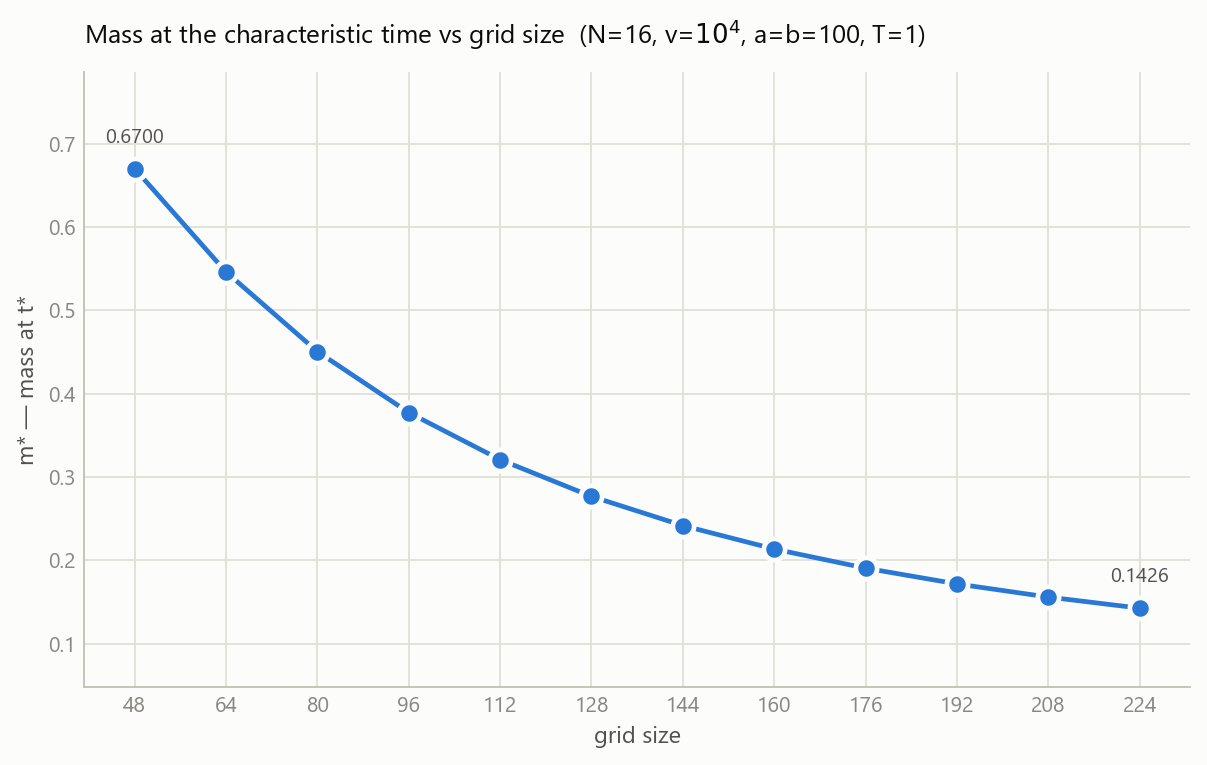
\includegraphics[width=\textwidth]{mass_vs_grid_size.png}
\end{center}

\end{document}
